\documentclass[11pt,letterpaper]{article}
\usepackage[lmargin=1in,rmargin=1in,tmargin=1in,bmargin=1in]{geometry}
\usepackage{../style/homework}
\usepackage{../style/commands}
\setbool{quotetype}{true} % True: Side; False: Under
\setbool{hideans}{true} % Student: True; Instructor: False

\newcommand{\blank}[1]{\underline{\hspace{#1}}} % Blank Underline

% -------------------
% Content
% -------------------
\begin{document}

\homework{10: Due 11/10}{Matrices act. They don't just sit there.}{Gilbert Strang}

% Problem 1
\problem{10} Showing all your work, compute the following:
	\begin{enumerate}[(a)]
	\item $\displaystyle \sum_{k=0}^5 (5k - 3)$
	\item $\displaystyle \sum_{\substack{k= -2 \\ k \neq 0}}^3 \dfrac{k + 1}{k}$
	\item $\displaystyle \prod_{j=1}^4 2j$
	\item $\displaystyle \prod_{n=2}^\infty \left(1 - \dfrac{1}{n^2} \right)$ \quad [Hint: Combine terms, then split the product.]
	\item $\displaystyle \sum_{k=1}^\infty \dfrac{1}{k^2 + 3k}$ \quad [Hint: Use partial fractions, then write out some terms.]
	\end{enumerate}

\newpage 
\begin{center} {\itshape --- Continued Space for Problem~1 ---} \end{center}
\newpage



% Problem 2
\problem{10} Define $\mathbf{u}= \langle 2, 0, -1, 3 \rangle$ and $\mathbf{v}= \langle 1, -1, 5, 6 \rangle$. Showing all your work, complete the following:
	\begin{enumerate}[(a)]
	\item $\mathbf{u} - 2 \mathbf{v}$
	\item $\| \mathbf{u} - 2\mathbf{v} \|$
	\item $\mathbf{u} \cdot \mathbf{v}$
	\item If $\mathbf{x}, \mathbf{y} \in \mathbb{R}^n$, then $\mathbf{x} \cdot \mathbf{y}= \| \mathbf{x} \| \, \| \mathbf{y} \| \cos \theta$, where $\theta$ is the angle between $\mathbf{x}$ and $\mathbf{y}$. Using this fact, compute the angle between $\mathbf{u}$ and $\mathbf{v}$. 
	\end{enumerate}



\newpage



% Problem 3
\problem{10} Define the following:
	\[
	A= \begin{pmatrix} 0 & -2 \\ 6 & 5 \end{pmatrix}, \qquad
	B= \begin{pmatrix} 1 & 0 & -1 & 3 \\ 5 & 1 & 0 & 4 \end{pmatrix}, \qquad
	C= \begin{pmatrix} 2 & 1 \\ -1 & 0 \\ 4 & 1 \\ -1 & 1 \end{pmatrix}, \qquad
	\mathbf{u}= \begin{pmatrix} 1 \\ -1 \end{pmatrix}
	\]
Showing all your work, compute the following:
	\begin{enumerate}[(a)]
	\item $BC - 2A$
	\item $CB$
	\item $B^T \mathbf{u}$
	\end{enumerate}



\newpage



% Problem 4
\problem{10} A \textit{neural network} is a computational model resembling how the human brain works and they are used to create predictive models in data science. There are many types of neural networks: feed-forward neural networks, recurrent neural networks, convolutional neural networks, etc. 
	\begin{enumerate}[(a)]
	\item Watch 3Blue1Brown's ``\href{https://www.youtube.com/watch?v=aircAruvnKk&list=PLZHQObOWTQDNU6R1_67000Dx_ZCJB-3pi&ab_channel=3Blue1Brown}{But what is a neural network?}'' and then comment about what you learned and how it relates to the course material. 
	\item Using sigmoid function $\sigma(x)= \frac{1}{1 + e^{-x}}$, bias vectors $\mathbf{b}_1= \begin{pmatrix} 1.5 \\ -0.4 \end{pmatrix}$ and $\mathbf{b}_2= \begin{pmatrix} 0.3 \\ 2.0 \end{pmatrix}$, and initial input $\mathbf{a}= \begin{pmatrix} 3 \\ -1 \end{pmatrix}$, compute the output of the single hidden layer neural network given below. 
		\[
		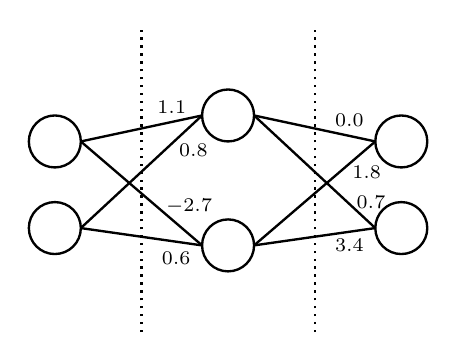
\begin{tikzpicture}[scale=1.1]
		% Input Layer
		\draw[line width=0.03cm] (0,0.2) circle (0.3);
		\draw[line width=0.03cm] (0,1.2) circle (0.3);
		% Hidden Layer
		\draw[line width=0.03cm] (2,0) circle (0.3);
		\draw[line width=0.03cm] (2,1.5) circle (0.3);
		% Output Layer
		\draw[line width=0.03cm] (4,0.2) circle (0.3);
		\draw[line width=0.03cm] (4,1.2) circle (0.3);
		
		% Dotted Lines
		\draw[line width=0.03cm,dotted] (1,-1) -- (1,2.5);
		\draw[line width=0.03cm,dotted] (3,-1) -- (3,2.5);
		
		% First Layer Lines
		\draw[line width=0.03cm] (0.3,1.2) -- (1.7,1.5);
		\draw[line width=0.03cm] (0.3,1.2) -- (1.7,0);
		\draw[line width=0.03cm] (0.3,0.2) -- (1.7,1.5);
		\draw[line width=0.03cm] (0.3,0.2) -- (1.7,0);
		
		% Second Layer Lines
		\draw[line width=0.03cm] (2.3,1.5) -- (3.7,1.2);
		\draw[line width=0.03cm] (2.3,1.5) -- (3.7,0.2);
		\draw[line width=0.03cm] (2.3,0) -- (3.7,1.2);
		\draw[line width=0.03cm] (2.3,0) -- (3.7,0.2);
		
		% Labels
		\node at (1.35,1.6) {\scriptsize$1.1$};
		\node at (1.6,1.1) {\scriptsize$0.8$};
		\node at (1.55,0.45) {\scriptsize$-2.7$};
		\node at (1.4,-0.15) {\scriptsize$0.6$};
		
		\node at (3.4,1.45) {\scriptsize$0.0$};
		\node at (3.6,0.85) {\scriptsize$1.8$};
		\node at (3.65,0.5) {\scriptsize$0.7$};
		\node at (3.4,0) {\scriptsize$3.4$};
		\end{tikzpicture}
		\]
	\end{enumerate}


\end{document}